\chapter{Asking Miami Millionaires How to Get RICH!}

These notes follow a School of Hard Knocks interview through Miami and treat it as a sequence of economic constructions rather than as a pile of motivational clips. The lecture begins with spectacle---huge years, huge months, stories of being broke, stories of coming back---and only gradually settles into mechanism. What finally emerges is a small but coherent bank of ideas: distressed entry when markets reset, the staged construction of an operator, the conversion of earned income into cash-flowing assets, the role of recurring revenue, and the slow hardening of habit. No validated blackboard frames survived review, so every displayed formula below is a cautious transcript-based reconstruction rather than a transcription of visible notation.

\begin{remark}
The lecture is numerically dense, but its numbers are interview claims. We use them as evidence of scale and structure, not as audited measurements.
\end{remark}

\section{Opening Montage and the Search Problem}

The lecture opens before it argues. We hear of a \$24 million year, a \$2.9 million month, a \$12 million loss, a trip to Vegas with \$100, and a later year above \$100 million. The effect is deliberate. Wealth is introduced together with volatility, humiliation, and recovery, so that the chapter begins with tension rather than with doctrine.

Only after this cold open does the host tell us what sort of object we are looking at. Miami is named as a dense field of millionaires, and the lecture adopts a repeatable method: identify the industry, pin down the scale, ask whether the person has ever been broke, and then try to extract a usable mechanism from the answer. The host's role is not only to ask for numbers. It is to turn one biography after another into a sequence of economic examples.

\begin{table}[h]
\centering
\begin{tabular}{lll}
Case & Claimed peak quantity & Quoted magnitude \\
Opening / Wes Watson & best year & \$24 million \\
Opening / Wes Watson & best month & \$2.9 million \\
Patrick (real estate) & best year & over \$100 million \\
E-commerce operator & best year & \$9.7 million \\
Later operator & best month & \$550{,}000 \\
Patrick (gross asset volume) & lifetime scale & over \$20 billion \\
\end{tabular}
\end{table}

The lecture also leans on a broader abundance claim:
\begin{equation}
N_{\mathrm{new/day}} = 1700.
\end{equation}
Here \(N_{\mathrm{new/day}}\) is the quoted number of new millionaires created every day. We should not turn this into a proved statistic. Its function in the lecture is motivational: wealth is framed as a recurring event, not as a mythical exception.

\section{Patrick: Real Estate at Scale, Then Real Estate Under Pressure}

The first full case belongs to Patrick, and the host moves exactly in the order promised by the opening frame. First industry: real estate. Then scale: buying and selling more than \$20 billion of assets, with roughly \$12 billion of apartments bought and roughly \$18--\$19 billion sold. Then personal extraction: S-corp returns at a level above \$100 million in a year, hitting the personal balance sheet because he owns the business.

We can formalize the scale just enough to make the lecture's arithmetic legible. Let \(V_b\) denote gross bought value and \(V_s\) gross sold value. Then the quoted magnitudes are
\begin{align}
V_b &\approx 12\times 10^9,\\
V_s &\approx (18\text{--}19)\times 10^9.
\end{align}

\paragraph{Worked example.} The lecture does not give us a capital stack, so we do not pretend to know return on equity or internal rate of return. What it does give us is a gross turnover marker:
\begin{equation}
\tau = \frac{V_s}{V_b} \approx \frac{18}{12}\text{--}\frac{19}{12} \approx 1.50\text{--}1.58.
\end{equation}
This \(\tau\) is only a sale-to-purchase scale ratio. It tells us that the speaker is narrating a very large real-estate machine, not that we have reconstructed its profitability in any rigorous sense.

The lecture then pivots hard. Right after scale comes fragility. Patrick says he became a millionaire around twenty-five, but he also says he remembers going to the ATM on Friday, pulling out money before the account went red, and living through the weekend by moving cash across multiple single-family construction deals. He himself describes it as robbing Peter to pay Paul. The host lets that memory stay in place long enough for it to do its work: success is no longer a static noun, but something built while managing pressure, shortage, and fear.

That fear is not treated as an embarrassment. It becomes a principle. If one has never felt broke, says Patrick, perhaps one has never acquired a healthy enough fear. The lecture's first case therefore establishes two things at once. Wealth can sit on top of gigantic asset turnover. But it can also grow out of a period in which the operator is simply trying to keep the machine from seizing up.

\subsection{Question \& Answer}

\paragraph{Question.} If the rich get richer and the poor get poorer, how does someone with very little capital actually get in?

\paragraph{Answer.} The lecture answers by changing the market picture before it changes the person. We are told that there is a ``huge reset in wealth'' because interest rates have pushed a wide class of financial assets down by something like \(30\%\) to \(40\%\). Let \(\delta\) denote that quoted drawdown fraction. Then the lecture's market condition may be normalized as
\begin{align}
\delta &\approx 0.30\text{--}0.40,\\
P_{\mathrm{now}} &\approx (1-\delta)P_{\mathrm{prior}}.
\end{align}

This is not meant as a universal law of valuation. It is a strategic snapshot. The lecture's argument is that when asset prices are down at that scale, lenders, owners, and operators are dealing with distress. A distressed market does not merely lower prices; it increases the value of anyone who can solve an operational problem.

That is why the lecture next replaces a capital-first story with a solution-first story. One does not necessarily begin by owning the whole asset. One begins by stepping into a neglected problem and taking a share of the upside. If \(\Pi\) is total project profit and \(\rho\) is the agreed share, the spoken example is
\begin{equation}
\Pi_{\mathrm{operator}} = \rho\,\Pi,\qquad \rho = 0.10.
\end{equation}

This is still only an example, but it reveals the mechanism clearly. The host is told to look for actual channels of entry:
\begin{enumerate}
\item work with lenders;
\item look at foreclosure situations;
\item take on ignored single-family houses through management or repositioning;
\item solve the problem in exchange for a share of profits;
\item or attach oneself to a wealthy operator and get pulled into deals from the side.
\end{enumerate}

The line that governs the whole answer is the inversion, ``capital is not needed right now; solutions are.'' We should keep that sentence exactly in its strategic spirit. It is not an eternal theorem about business. It is a claim about what becomes valuable when markets are stressed.

The host's recap is then important. He does not merely celebrate Patrick's size. He traces the personal income back to the real-estate machine, and the machine back to repeated transactions at very large scale. That is the lecture's first complete unit: scale, fear, distressed entry.

\section{The E-Commerce Ladder and the Command to Act}

The next interview changes industries without changing the lecture's deeper method. The speaker is in e-commerce, has been in the business since 2018, and reports a best year of \$9.7 million. But once again the host refuses to stop at the number. He asks how the business scaled and what went wrong earlier.

The answer comes as a staged ladder. The speaker says he went broke three times, and that each failure exposed a missing capacity. The lecture's cleanest operator progression appears here:
\begin{equation}
\text{Branding}\rightarrow 10^6,\qquad
\text{Marketing}\rightarrow 10^7,\qquad
\text{Systems}\rightarrow 10^8.
\end{equation}

We should read this with care. It is not a universal law of commerce. It is a retrospective decomposition of what that particular operator thinks each order of magnitude demanded. Yet it is exactly the sort of quasi-formal statement the lecture wants us to retain. In Patrick's case, the mechanism was distressed entry into real estate. Here the mechanism is staged operator construction.

The lecture then widens again, this time from business mechanics to civic insistence. The speaker returns to the 1{,}700-millionaires-per-day claim, says he himself became one on a random Tuesday, remembers working for \$8 an hour, remembers cheap cars that broke down, remembers walking to work, remembers collapsing on the pavement with nobody stopping to help, and concludes that nobody is coming to save us. The host then distills the whole segment into a short imperative: just take action.

The order matters. First the ladder. Then the civic and psychological interpretation. If we invert those, we flatten the lecture into anonymous mindset talk. As spoken, the lecture wants us to feel that courage without method is too soft, and method without urgency is too inert.

\section{From Earned Income to Financial Freedom}

Eric Spofford's appearance is the conceptual center of the lecture. He reports a year above \$100 million, but that headline is immediately subordinated to a more serious question: why do people stay trapped even after they start making serious money?

\begin{definition}
In the lecture's operational language, \emph{financial freedom} is the regime in which present lifestyle is funded from the cash flow of appreciating assets rather than from raw current earned income.
\end{definition}

To make that mechanism explicit, let \(Y_t\) be earned income at time \(t\), \(L_t\) direct lifestyle spending, \(s_t\) the amount retained and reinvested, \(A_t\) the stock of cash-flowing appreciating assets, and \(C_t\) the cash flow produced by that stock. Then the lecture's logic may be written as
\begin{align}
Y_t &= L_t + s_t,\\
A_{t+1} &= A_t + s_t,\\
C_t &= C(A_t),\\
L_t &\approx C_t.
\end{align}

The first line says that earned income is not itself the endpoint; it is the input to an allocation decision. The second says that retained income becomes an asset stock. The third says that the asset stock throws off cash. The fourth captures the lecture's intended regime: one does not keep funding life from immediate earned income if one can instead fund it from the flow of an accumulated asset base.

\subsection{Question \& Answer}

\paragraph{Question.} What is the common mistake that keeps people poor after they have started making money?

\paragraph{Answer.} The lecture answers with the phrase ``poor mindset,'' but the content is quite concrete. People make money, then consume it as if it were proof rather than feedstock. They spend it on dinners, cars, accessories, expensive housing, and the symbolic rewards of having made it, while failing to turn present earnings into future-producing assets.

That is why Eric repeats the mechanism more than once. Make the money. Do not spend the whole thing as lifestyle. Put the retained portion into what he calls cash-flowing appreciating assets. Then live off the generated cash flow. If one does not yet know what that phrase means, he says, one is already in trouble. The lecture is not trying to define terms for elegance; it is trying to force a sequence into memory.

We may summarize the preferred structure in a transcript-derived schematic:

\begin{figure}[h]
\centering
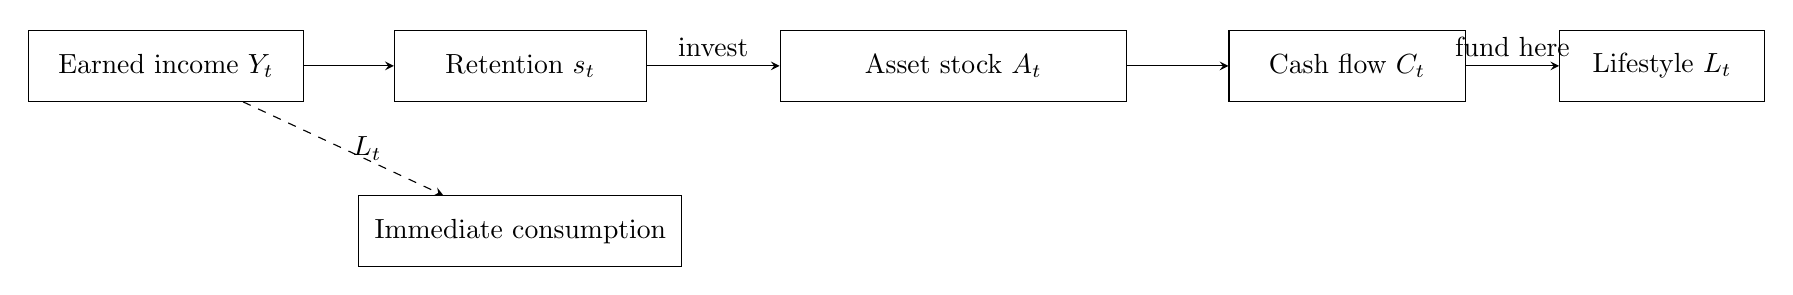
\begin{tikzpicture}[>=stealth]
\node[draw, rectangle, minimum width=3.5cm, minimum height=0.9cm] (Y) at (0,0) {Earned income \(Y_t\)};
\node[draw, rectangle, minimum width=3.2cm, minimum height=0.9cm] (S) at (4.5,0) {Retention \(s_t\)};
\node[draw, rectangle, minimum width=4.4cm, minimum height=0.9cm] (A) at (10.0,0) {Asset stock \(A_t\)};
\node[draw, rectangle, minimum width=3.0cm, minimum height=0.9cm] (C) at (15.0,0) {Cash flow \(C_t\)};
\node[draw, rectangle, minimum width=2.6cm, minimum height=0.9cm] (L) at (19.0,0) {Lifestyle \(L_t\)};
\node[draw, rectangle, minimum width=4.1cm, minimum height=0.9cm] (D) at (4.5,-2.1) {Immediate consumption};

\draw[->] (Y) -- (S);
\draw[->] (S) -- node[above] {invest} (A);
\draw[->] (A) -- (C);
\draw[->] (C) -- node[above] {fund here} (L);
\draw[->, dashed] (Y) -- node[right] {\(L_t\)} (D);
\end{tikzpicture}
\end{figure}

The dashed lower path is the lecture's warning. The solid upper path is its preferred economic construction. The endpoint is also given a social name: not status, but independence---the lecture's rough phrase for this is \emph{fuck-you money}.

\section{Roadmap, Expertise, and the Correct Time Asymmetry}

From allocation the lecture passes to design. The host now asks how someone becomes wealthy going into 2024, and the answer turns away from mere hustle language toward structure: find your thing, build a blueprint, have a roadmap, do not move without a design.

The essential point is temporal. The lecture insists that people misjudge not only the amount of work required but the horizon on which that work must sit. The speaker says he already knows what he is doing month over month for the next five years. That is not presented as an eccentric trait; it is presented as part of the wealth machine itself.

The contrast is delivered almost as a pair of equations:
\begin{align}
\text{winning posture} &= \text{macro patience} + \text{micro urgency},\\
\text{failure posture} &= \text{micro patience} + \text{macro urgency}.
\end{align}

This is not algebra in any literal sense. It is a compact asymmetry. The lecture's complaint is that people reverse the two scales. They demand the large outcome too quickly and then behave too softly in the day-to-day moves. The right posture is the opposite: patient at the horizon, urgent in the daily step.

The host's recap then adds one more guardrail: become an expert and the best in the world at one thing, or be slaughtered in business. We should not smooth this into bland specialization advice. In the lecture it functions as a boundary condition. Without one thing, one plan, and one horizon, the entrepreneur dissipates force.

The next, rougher interview reinforces the same warning from a different angle. A speaker who reports a best month of \$550{,}000 and remembers losing \$12 million in a year rejects the idea that poverty is a fixed cycle. But his more durable point is about temporality: do not go crazy with money, because some earning streams end. Athletes are the example. The money can be large and the horizon short. If there is no design after the income spike, the spike is not freedom.

\section{Recurring Revenue and the Hardening of Habit}

The lecture's last full case belongs to Wes Watson. Once more we begin with the familiar rhythm: past broke state, present scale, then mechanism. Wes recalls prison and extreme scarcity, then reports the by-now familiar headline numbers of \$24 million in a year and \$2.9 million in a month. But the host asks a more useful question: how does one move from seven to eight figures?

The answer begins socially. Get around people who are operating at a larger scale, people for whom very high monthly expenses are normal, people who use money as a tool rather than as a trophy. That answer then sharpens into a distinction the lecture cares about deeply. Many people talk only about passive income. Wes insists instead on the importance of earned income at the top of the game.

The lecture then compresses one major business principle into a slogan: the ``double R'' stands for recurring revenue. In the smallest possible notation we may write
\begin{equation}
R_t > 0
\end{equation}
throughout the operating horizon. The point is not that this is a full revenue model. The point is that repeated inflow is structurally different from isolated wins. The lecture wants us to see recurring revenue as something built, defended, and renewed.

Only after that does the final blueprint arrive. We are told not merely to do what one loves, but to work for what one wants, choose a path by looking at the people one wants to resemble, and refuse the comfort of waiting for permission. Wes's prison-to-Instagram story is the lecture's closing example of long-horizon consistency: seeing the platform early, posting through confinement, leaving prison with an audience, and then never missing. The lecture now shifts almost completely from money to recurrence.

If we want a compact editorial way to display that final point, we may write
\begin{equation}
H_{t+1} = H_t + h_t,
\end{equation}
where \(h_t\) is a day's package of repeated actions: posting, training, waking early, serving others, and keeping promises. This is not a spoken equation from the lecture. It is a modest reconstruction of the repeated update rule that the lecture narrates in words.

The closing details matter. Rising at 2:45. Training every day, often more than once. Keeping nutrition tight. Serving others. The lecture ends here because at the far end of all the money talk it wants to leave us with a stricter thought: wealth is not merely the possession of a large number. It is the stabilization of a pattern.

\section{Summary}

The lecture begins by throwing numbers at us, but it ends by organizing them. Patrick gives us real-estate turnover, cash stress, and distressed entry through solutions. The e-commerce operator gives us a stage ladder: branding, then marketing, then systems. Eric Spofford gives us the cleanest formal mechanism in the chapter: earned income should be split, retained, converted into cash-flowing appreciating assets, and eventually replaced by the cash flow those assets generate. The later interviews harden the horizon problem and finally shift us toward recurring revenue and daily recurrence.

So the mathematical payload of the chapter is limited, but it is real. We have a gross turnover ratio, a drawdown fraction, a profit-share template, an income-allocation rule, a cash-flow description of freedom, and a compact contrast between the right and wrong pairing of patience and urgency. None of this is blackboard mathematics. All of it, however, is part of the lecture's deliberate progression.

If we ask what the lecture finally believes, the answer is not mysterious. Wealth is built by entering where problems are real, by constructing the operator, by refusing to consume every win as proof, by turning earned income into productive assets, by designing for the long horizon, and by repeating the daily acts long enough for them to become a machine.